\chapter{Implementation}
\label{implementation}

The project is implemented using Object Oriented Programming paradigm, where objects represent elements displayed on the screen, haptic elements and controllers. The application has two threads - one for graphic and one for haptic calculations and operations. Graphic thread is working as a loop with about 60 Hz frequency, where haptic's frequency is around 1000Hz. 

\section{Haptic devices}
At it was mentioned in \emph{\ref{phantom_introduction} : \nameref{phantom_introduction},} the haptice device chosen for this application is Sensable Phantom Omni. It was chosen for this project because of common usage of this device in similar experiments and projects \cite{13}.

\section{Programming language and libraries}
In order to create a game, there is a need to choose the two main libraries - graphic and haptic one. Additional dependencies like audio library or model loader won't be present in this version of the application. The programming language should be compatible with both of libraries. 

\subsection{Graphic library}
The graphic library that has been chosen is \textbf{OpenGL}. The main reason for such a decision is support from haptic dependencies for this library. Another arguments for this choice are: 
\begin{itemize} [noitemsep]
\item portability
\item personal experience
\end{itemize}
Another possibilities were: DirectX library and OpenGL-based haptic libraries. The latter was rejected because of poor manual available and the former - because of worse compatibility with haptic device.

\subsection{Haptic library}
\begin{wrapfigure}{R} {0.5\textwidth}
\begin{center}
	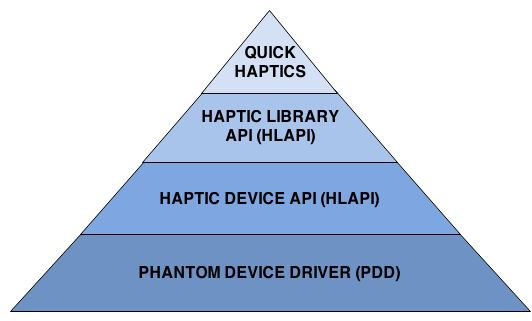
\includegraphics[width=5cm]{Images/open_haptics}
	\caption{Description of Open Haptic APIs}
	\label{fig:haptics_api}	
\end{center}
\end{wrapfigure}
Two most popular libraries for usage with Phantom Omni are Open Haptics (from Phantom's manufacturer) and Open Source H3DAPI(from SenseGraphics). 

Open Haptics is based on OpenGL using C/C++ and is available under two types of licence: academic and commercial. This library provides well written manual and programmer's guide as well as API description and examples. It consist of three separate APIs, each on different level of abstraction, as described in the figure\emph{ \ref{fig:haptics_api} : \nameref{fig:haptics_api}}(the lowest level is the device driver). Quick Haptics is the most abstract API and allows quick development of application with limited user customisation. Haptic Device API is the lowest-level one and gives direct access to the haptic device together with possibility of independent generating haptic forces. Medium one, Haptic Library API, is used together with standard OpenGL applications as an "haptic addition", that allows to generate haptic objects from not-haptic user objects, but does not give such a low-level access as HDAPI.

Open Source H3DAPI is a software developed by SenseGraphics and its community. It is based on X3D, C++(OpenGL) and Python. It is high-level API that helps in haptic and graphic rendering. Unfortunately, the available manuals and documentation are very meagre. H3DAPI has its own application architecture, different than typical OpenGL application structure, so OpenGL code and experience cannot be reused while using this API. Application that uses Open Haptics can be developed separately by OpenGL developers and haptic developers. It is much harder with H3DAPI. Moreover, it is easier to teach OpenGL specialist Open Haptics than H3DAPI.

Then, the library of choice is \textbf{Haptic Library API} (under Academic Licence), because of following reasons:
\begin{itemize} [noitemsep]
\item fast consolidation with working OpenGL applications
\item well described documentation and examples
\item level of abstraction low enough to perform minor customisation, but also high enough to avoid excessive control over haptic device
\end{itemize}

\subsection{Programming language}
Programming language used in the project is \textbf{C++}. It is prime language to use with OpenGL and is suggested language to use with Open Haptics. What is more, it allows necessary optimisation together with applying OOP paradigm.

\subsection{Code samples} 
Some of the functions and solutions used in the application are based on single functions from Angel's OpenGL API and Sensable Open Haptics examples.

\section{Other used programming tools}
While developing an application, choosing the additional tools is as important as choosing libraries and APIs. The following tools are taken under consideration: IDE and version control system.

\subsection{IDE}
As the application is developed under Microsoft Windows 7 operating system, Microsoft Visual Studio 2010 is IDE of choice. It is advanced and convenient IDE for C++ programming under Windows OS. The version 2010 was chosen because of its stability and compatibility with Open Haptics as well as because of personal experience. 

\subsection{Version control}
Distributed version system has been chosen, because of its clear advantage over not-distributed (each user has his own copy of full repository). The used version control system is Mercurial with TortoiseHg Windows client. 

\section{Components}
The main application components dependencies are described in figure \emph{\ref{fig:component} : \nameref{fig:component}}. 
\begin{itemize} [noitemsep]
\item \emph{Controllers} - package name for \emph{\ref{controllers} : \nameref{controllers}}. Responsible for game logic and updating objects' properties.
\item \emph{Haptic thread} - abstract name for both implemented and embedded functionalities of haptic API. Responsible for collision testing, generating feedback based on haptic objects' properties to device and passing the current position value. 
\item \emph{Haptic device} - physical Phantom Omni device, receiving feedback parameters from application and sending back the current position.
\item \emph{Graphic thread} - abstract name for both implemented and embedded functionalities of graphic API. Responsible for rendering the display based on object's properties. 
\item \emph{Mouse} - physical input from mouse, received by Controllers.
\item \emph{Keyboard} - physical input from keyboard, received by Controllers.
\end{itemize}

\begin{figure}
\begin{center}
	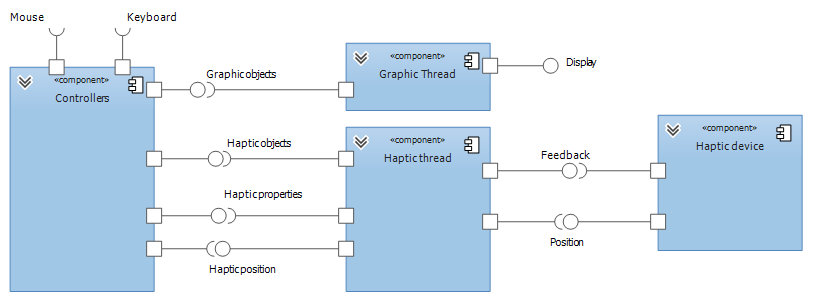
\includegraphics[width=\textwidth]{Images/component_diagram}
	\caption{Components diagram}
	\label{fig:component}	
\end{center}
\end{figure}


\section{Data flow}
\begin{figure}
\begin{center}
	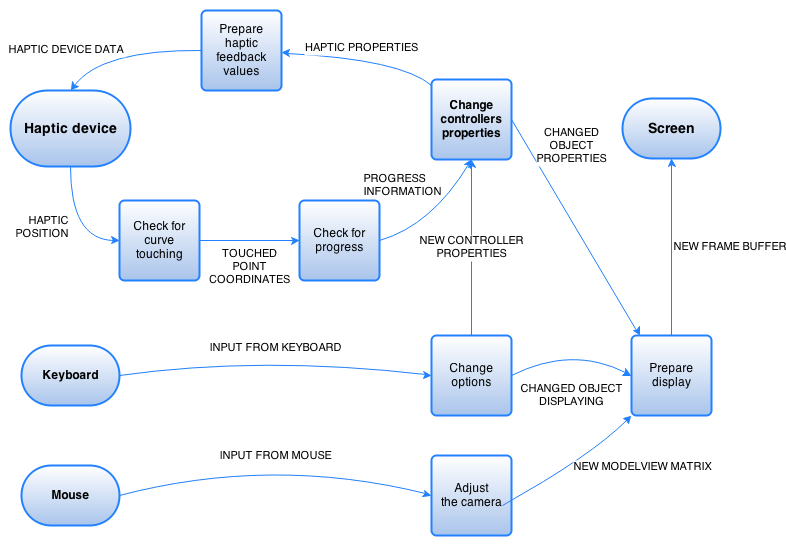
\includegraphics[width=\textwidth]{Images/data_flow_diagram}
	\caption{Data flow diagram}
	\label{fig:flow}	
\end{center}
\end{figure}
Figure \emph{\ref{fig:flow} : \nameref{fig:flow}} presents the flow of information in the application. 


\section{Class structure}
\label{class_structure}
Simplified class diagram is presented in figure \emph{\ref{fig:class} : \nameref{fig:class}}. It presents the most important classes of the program and their dependencies. It does not contain all methods and fields - mathematical and some of private objects and functions are skipped in order to keep the diagram legible. Also, application uses some functions designed for graphical thread which are not presented in the diagram, but described in the following subsections.  
\begin{figure}
\begin{center}
	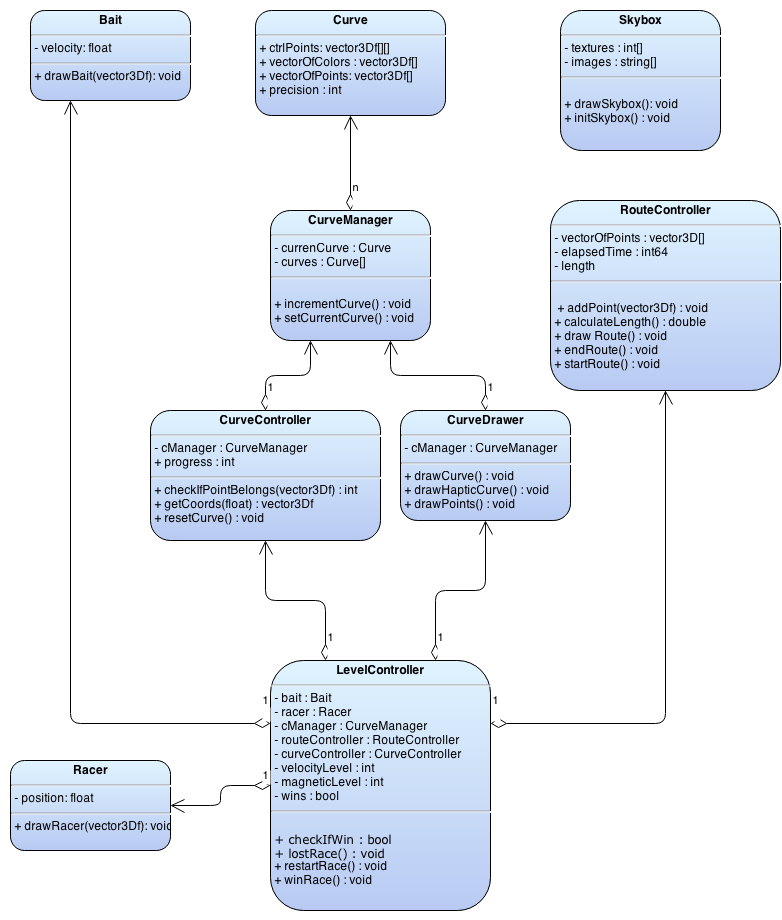
\includegraphics[width=\textwidth]{Images/class_diagram}
	\caption{Class diagram}
	\label{fig:class}	
\end{center}
\end{figure}

\subsection{Data structures}
For application usage the following data structures were create:
\begin{itemize} [noitemsep]
\item \emph{Curve} - storing path details like: control points (for Bezier's curve), total race time (slow and fast).
\item \emph{Skybox} - loads six skybox textures and keep skybox cube parameters.
\item \emph{Bait} - competitor's object.
\item \emph{Racer} - player's object
\item \emph{RouteController} - collects data about player's score.
\end{itemize}

\subsection{Initialization} 
In order to properly initialize graphic and haptic thread, three functions were designed:
\begin{itemize} [noitemsep]
\item \emph{initGL()} - setting the lighting, defining OpenGL properties and initializing Skybox.
\item \emph{initHL()} - initializing the haptic device, setting proper callbacks for haptic objects.
\item \emph{initObject()} - initializing game objects.
\end{itemize}

\subsection{Drawing components}
\label{drawing_components}
The following components interact with graphic thread and draw to the graphic buffer:
\begin{itemize} [noitemsep]
\item \emph{CurveDrawer} - draws the path and/or path control points.
\item \emph{Bait} - draws the Bait.
\item \emph{Racer} - draws the Racer.
\item \emph{RouteController} - if proper mode is enabled, draws the player's route.
\item \emph{Skybox} - if proper mode is enabled, draws the Skybox.
\item \emph{drawCursor()} - draws cursor representation based on current proxy position.
\item \emph{drawSceneGraphics()} - calls all the other drawing functions and sets their properties.
\item \emph{drawMessage()} - draws message on the screen.
\end{itemize}

\subsection{Haptic components}
Haptic componenents are classes and functions that communicates with haptic thread and device. 
\begin{itemize} [noitemsep]
\item \emph{CurveDrawer} - draws the path to the haptic buffer. 
\item \emph{drawSceneHaptics()} - main function responsible for setting haptic properties and calling all the other functions that draws to haptic buffer.
\item \emph{updateHapricMapping()} - maps haptic device workspace to world coordinates after camera properties changes. 
\item \emph{TouchCollisionThreadCallback()} - called when Curve is touched.
\item \emph{UnTouchCollisionThreadCallback()} - called when Curve stopped to be touched. 

\end{itemize}

\subsection{Controllers}
\label{controllers}
Controllers represent the game logic. 
\begin{itemize} [noitemsep]
\item \emph{CurveManagaer} - keeps track of current Curve and stores all the others.
\item \emph{CurveController} - checks for collisions with cursor and generate coordination based on 0-1 float number (0 - start of the Curve, 1 - end of the Curve).
\item \emph{RouteController} - measures the player's path and calculate length and time of race.
\item \emph{LevelController} - responsible for win checking, passing to another level and updating all the other controllers.
\item \emph{glutKeyboard()} - function responsible for grabbing input from keyboard and calling appropriate function when key pressed.
\item \emph{glutMouse()} - function responsible for detecting mouse buttons' pressing and setting appropriate control values. 
\item \emph{glutMotion()} - function responsible for measuring mouse motion and setting appropriate camera values, if mouse buttons are pressed. 
\end{itemize}

\subsection{Camera}
Camera is not represented as seperate class in program, however it has predefined global properties that can be changed with mouse. Camera properties are updated by keyboard and mouse functions and applied to modelView matrix in the following functions: 
\begin{itemize} [noitemsep]
\item \emph{glutReshape()} - initialises modelView matrix and updates it after window reshaping.
\item \emph{updateCamera()} - updates modelView matrix after camera properties change.
\end{itemize}

\section{Implementation details}
This section is focused on parts of code that require additional explanation or description. 
\subsection{Path graphical and haptic representation}
\label{path_representation}
Path is depicted with Bezier's curve. However, while drawing it, application evaluates some finite number of points that belongs to curve and uses them to draw it. Number of points is defined by precision attribute of CurveController (its value is about 1000).
Displayed path consists of small beads (spheres),where each bead represents one point of a curve. Haptic path representation is a line strip between those points. The reasons are simple:
\begin{enumerate} [noitemsep]
\item {Necessity for differences in precision value.}

The precision for haptic path is smaller than for displayed one in order to keep the path smooth in touch - haptic thread frequency is 1000Hz and if it has to test too high (from tests - around 500) number of objects, it acts like the surface it touches is rough and it is hard to move the stylus along the path. However, it its important to remember, that precision for haptic cannot be too low - the haptic and displayed path can differentiate in shape in such case.

\item {Necessity for differences in points connecting method.}

The basic way of connecting the points is using OpenGL property GL\_LINE\_STRIP. While adding vertices (points) to a buffer of the path shape, each new point is connected with the last added by line. Obtained line has no depth - light has no influence on this shape, which means that it's color is uniform and give no clues about distance or depth. This problem can be solved if each point is represented as a shape - in this case, the sphere. Lighting works on spheres and moreover, this solution makes the path looks like a string of beads, which is much more attractive for children than casual line.

\end{enumerate} 

\subsection{Progress detecting}

Progress detecting is a process that repeat with 50 Hz frequency. It has to determine if the player is able to move his object or not by detecting the collision of path, cursor and the object. 

The information, that player is touching the path, comes from haptic thread. It has appropriate properties set if such event is happening. The problem is in checking on which part of path play is now. The whole path cannot be checked during the short time (not even 20 ms) because it would require checking collision with even 500 elements that path consists of (the path construction was described in subsection above). The approximation is used, that in current moment of time application tests only 10 elements (points) that lied on the path just in front of the player's object - if the cursor "collide" with any of this points, object is moving to this point and procedure is repeated until end of path. 
